% Article type supporting font formatting
\documentclass[a4,12pt]{extarticle}

% Define .tex file encoding
\usepackage[utf8]{inputenc}

% Norwegian language support
%\usepackage[norsk]{babel}     

% Indent first paragraph in section
\usepackage{indentfirst}

% Allows mathbb in tex file
\usepackage{amsfonts}    
     
% Margin defining package
\usepackage{geometry}         
\geometry{a4paper
  ,margin=1in
}

\usepackage[square,numbers]{natbib}

% For use of graphics in document
\usepackage{graphicx}         

% Allows multi-line comments in tex file
\usepackage{verbatim}         

% Allows math in tex file 
\usepackage{amsmath}          

% Allows math symbols in tex file
\usepackage{amssymb}          

% Allows use of physics shortcut functions
%\usepackage{physics}          

% Verbatim env with LaTeX commands
\usepackage{alltt}            

% Allows \begin{figure}[H]
\usepackage{float}            

% Necessary for defining colours
\usepackage{color}            
\definecolor{linkgreen}{rgb}{0,.5,0}
\definecolor{linkblue}{rgb}{0,0,.5}
\definecolor{linkred}{rgb}{.5,0,0}
\definecolor{blue}{rgb}{.13,.13,1}
\definecolor{green}{rgb}{0,.5,0}
\definecolor{red}{rgb}{.9,0,0}

% Hyperlinks in document
\usepackage{hyperref}  
\hypersetup{
  colorlinks=true,     % True for colored links
  linktoc=all,         % True for table of contents links
  linkcolor=linkblue,  % Colour for links
  urlcolor=linkgreen,  % Colour for URLs
  citecolor=linkred    % Colour for citations
}

% Listing package for code examples
\usepackage{listings}         
\lstset{
  language=C++,                % Set language to C++
  showspaces=false,            % Don't show space chars
  showtabs=false,              % Don't show tab chars
  breaklines=true,             % Break long lines of code
  showstringspaces=false,      % Don't show spaces in strings
  breakatwhitespace=true,      % Break at white space only
  commentstyle=\color{green},  % Set colour for comments
  keywordstyle=\color{blue},   % Set colours for keywords
  stringstyle=\color{red},     % Set colour for strings
  basicstyle=\ttfamily,        % Set basic style
  tabsize=2                    % Set tabsize
}

% Referencing, last for compatibility reasons
\usepackage[noabbrev]{cleveref}

% Command to set two lines under text
\newcommand{\uunderline}[1]{\underline{\underline{#1}}}

% Command to use integral with limits
\newcommand{\Int}{\int\limits}    

% Command to use double integral with limits
\newcommand{\IInt}{\iint\limits}  

% Command to use triple integral with limits
\newcommand{\IIInt}{\iiint\limits}

% Command removes section numbering
\newcommand{\mysection}[2]{   
\setcounter{section}{#1}
\section*{#2}
\addcontentsline{toc}{section}{#2}
}

% Command removes subsection numbering
\newcommand{\mysubsection}[2]{  
\setcounter{subsection}{#1}
\subsection*{#2}
\addcontentsline{toc}{subsection}{#2}
}

% Command removes subsubsection numbering
\newcommand{\mysubsubsection}[2]{ 
\setcounter{subsubsection}{#1}
\subsubsection*{#2}
\addcontentsline{toc}{subsubsection}{#2}
}

% Makes matrices look square-ish
\renewcommand*{\arraystretch}{1.5}

%%%%%%%%%%%%%%%%%%%%%%%%%%%%%%%%%%%%%%%
%%      Title, Author, and Date      %%
%%%%%%%%%%%%%%%%%%%%%%%%%%%%%%%%%%%%%%%
\title{Assignment 7 in Artificial Intelligence\\Spring 2018 }
\author{Daniel Aaron Salwerowicz}
\date{\today}

%%%%%%%%%%%%%%%%%%%%%%%%%%%%%%%%%%%%%%%
%%           Start document          %%
%%%%%%%%%%%%%%%%%%%%%%%%%%%%%%%%%%%%%%%
\begin{document}
  
%%%%%%%%%%%%%%%%%%%%%%%%%%%%%%%%%%%%%%%
%%   Create the main title section   %%
%%%%%%%%%%%%%%%%%%%%%%%%%%%%%%%%%%%%%%%
\maketitle

%%%%%%%%%%%%%%%%%%%%%%%%%%%%%%%%%%%%%%
%%  The main content of the report  %%
%%%%%%%%%%%%%%%%%%%%%%%%%%%%%%%%%%%%%%

\mysection{1}{Task 1}
\mysubsection{1}{1.1}
In nature a pheromone is a chemical substance left by ants to inform other ants which path to follow. In computer science instead of chemical substances we use numerical values to represent pheromones. The more pheromones (higher pheromone value) are left on a specific path, the more likely is it that other ants will choose given path instead of wandering at random. In turn leaving their own pheromones there (increasing the pheromone value). Pheromones evaporate over time (pheromone value decreases) therefore a longer path means that pheromones left on it have more time to evaporate than on shorter route. Shorter route makes it possible for more ants to travel quickly back and forth, leaving even more pheromones. This means that soon all or almost all ants will choose the best path as long as it gives the positive results.

\mysubsection{2}{1.2}
\mysubsubsection{1}{a}
Using the formula: $$P=\frac{\tau(r,u)^\alpha \cdot \eta(r,u)^\beta}{\sum_{k=1}^{K}\tau(r,k)^\alpha \cdot \eta(r,k)^\beta}$$ I calculate which path will be chosen using values: $\alpha=\beta=0.9$. $\tau(r,u)$ is simply the amount of pheromones on path $r\rightarrow u$ and $\eta(r,u)$ is the desirability of path given by $\frac{1}{d(r,u)}$, $d(r,u)$ is the distance between $r$ and $u$. $\alpha$ and $\beta$ are heuristic weights given to pheromone level and distance respectively and they vary between 0 and 1.

\begin{align*}
P(a,b) &= \frac{\tau(a,b)^\alpha \cdot \eta(a,b)^\beta} {\sum_{k=1}^{K} \tau(a,k)^\alpha \cdot \eta(a,k)^\beta}\\
&= \frac{2^{0.9} \cdot \frac{1}{8}^{0.9}}{2^{0.9} \cdot \frac{1}{8}^{0.9}+3^{0.9} \cdot \frac{1}{10}^{0.9} + 1^{0.9} \cdot \frac{1}{4}^{0.9}+2.5^{0.9} \cdot \frac{1}{7}^{0.9}}\\
&= \underline{0.2194505374}\\
P(a,c) &= \frac{\tau(a,c)^\alpha \cdot \eta(a,c)^\beta} {\sum_{k=1}^{K} \tau(a,k)^\alpha \cdot \eta(a,k)^\beta}\\
&= \frac{3^{0.9} \cdot \frac{1}{10}^{0.9}}{2^{0.9} \cdot \frac{1}{8}^{0.9}+3^{0.9} \cdot \frac{1}{10}^{0.9} + 1^{0.9} \cdot \frac{1}{4}^{0.9}+2.5^{0.9} \cdot \frac{1}{7}^{0.9}}\\
&= \underline{0.2585828812}\\
P(a,d) &= \frac{\tau(a,d)^\alpha \cdot \eta(a,d)^\beta} {\sum_{k=1}^{K} \tau(a,k)^\alpha \cdot \eta(a,k)^\beta}\\
&= \frac{1^{0.9} \cdot \frac{1}{4}^{0.9}}{2^{0.9} \cdot \frac{1}{8}^{0.9}+3^{0.9} \cdot \frac{1}{10}^{0.9} + 1^{0.9} \cdot \frac{1}{4}^{0.9}+2.5^{0.9} \cdot \frac{1}{7}^{0.9}}\\
&= \underline{0.2194505374}\\
P(a,e) &= \frac{\tau(a,e)^\alpha \cdot \eta(a,e)^\beta} {\sum_{k=1}^{K} \tau(a,k)^\alpha \cdot \eta(a,k)^\beta}\\
&= \frac{2.5^{0.9} \cdot \frac{1}{7}^{0.9}}{2^{0.9} \cdot \frac{1}{8}^{0.9}+3^{0.9} \cdot \frac{1}{10}^{0.9} + 1^{0.9} \cdot \frac{1}{4}^{0.9}+2.5^{0.9} \cdot \frac{1}{7}^{0.9}}\\
&= \underline{0.3025160441}\\
\end{align*}

Since $\alpha$ and $\beta$ give equal weight to pheromone level and distances we end up with solution that path $A \rightarrow E$ is most likely to be chosen.

\mysubsubsection{2}{b}
Using path from previous point I will calculate pheromone level left on the path by ant traveling across it. This is given by a formula: $$\tau_{i,j}(t)=(1-\rho)\tau_{i,j}(t-1) + \Delta \tau_{i,j}(k)$$ $\rho= 0.9$ and $Q=10$. $\Delta \tau_{i,j}(k)$ is the amount of pheromone left by the ant and it is given by $\Delta \tau_{i,j}(k)= Q \cdot \frac{1}{d(k)}$ where $Q$ stands for pheromone deposition capability, $d(k)$ is the length of path $k$. $\rho$ is the decay factor of the pheromone.

\begin{align*}
\tau_{a,e}(t) &=(1-\rho)\tau_{a,e}(t-1) + \Delta \tau_{a,e}(E)\\
             &=(1-0.9) 2.5 + 10 \cdot \frac{1}{7}\\
             &=\underline{1.678571429}
\end{align*}

Given probability that other paths may be chosen I have also calculated pheromone levels for them.

\begin{align*}
\tau_{a,b}(t) &=(1-\rho)\tau_{a,b}(t-1) + \Delta \tau_{a,b}(E)\\
             &=(1-0.9) 2 + 10 \cdot \frac{1}{8}\\
             &=\underline{1.45}\\
\tau_{a,c}(t) &=(1-\rho)\tau_{a,c}(t-1) + \Delta \tau_{a,c}(E)\\
             &=(1-0.9) 3 + 10 \cdot \frac{1}{10}\\
             &=\underline{1.3}\\
\tau_{a,d}(t) &=(1-\rho)\tau_{a,d}(t-1) + \Delta \tau_{a,d}(E)\\
             &=(1-0.9) 1 + 10 \cdot \frac{1}{4}\\
             &=\underline{2.6}\\
\end{align*}

From this we can see that if some ant decides to go to D its pheromone level would increase greatly and make it more probable that D will be chosen by other ants thus increasing its value. That is quite easy to believe since D has the shortest distance of 4 compared to others, which are  7, 8, 10.

\mysubsubsection{3}{c}
Values of $\alpha$ and $\beta$ decide how much weight is put on the pheromone and distance respectively when ant chooses the path it will take. If $\alpha$ is higher, then pheromone level will take precedence over distance and vice versa.

\mysection{2}{Task 2}
\mysubsection{1}{a}
The general shape of a perceptron can be seen in \cref{fig:Perceptron}. In our case it will have only two dendrites one for x value input and one for y value input. Dendrites is used to gather data while Axon sends data to synapses that connect to other Perceptrons.
\begin{figure}[H]
  \centering
  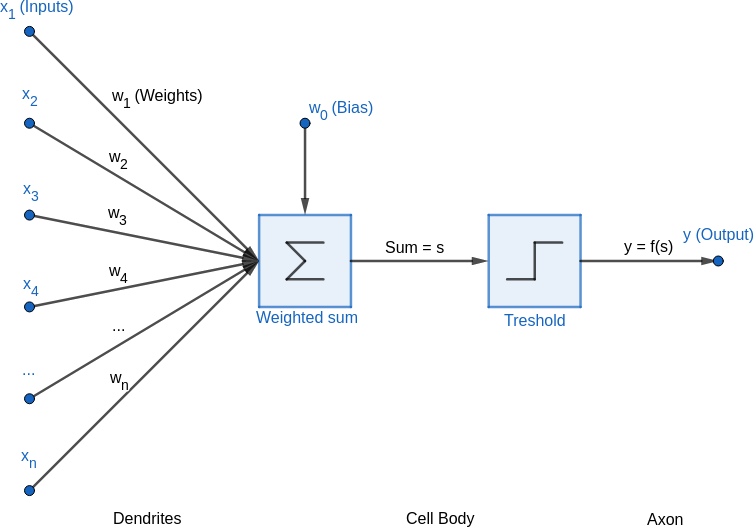
\includegraphics[width=0.7\textwidth]{Perceptron}
  \caption{General shape of a perceptron}
  \label{fig:Perceptron}
\end{figure}

\mysubsection{2}{b}
Since training and testing values are invalid (they are not linearly separable) I have taken liberty to change them so that they are separable. They can be seen in \cref{tab:TrainingValues,tab:TestingValues}.

\begin{table}[H]
  \centering
  \caption{Training Values}
  \label{tab:TrainingValues}
  \begin{tabular}{|l|l|l|l|l|l|l|l|l|}
    \hline
    \multicolumn{9}{|c|}{Category 1}            \\ \hline
    x & -10 & -10 & -9 & -5 & -3 &  2 &  5 &  5 \\ \hline
    y &   8 &  14 & 12 &  5 &  0 & -3 & -7 & -8 \\ \hline
  \end{tabular}
  \begin{tabular}{|l|l|l|l|l|l|l|l|l|l|}
    \hline
    \multicolumn{10}{|c|}{Category 2}           \\ \hline
    x &  5 & 5 & 4 & 1 & 1 & -2 & -3 & -6 & -10 \\ \hline
    y & -6 & 0 & 0 & 0 & 1 &  5 & 11 & 18 &  24 \\ \hline
  \end{tabular}
\end{table}
\begin{table}[H]
\centering
\caption{Testing Values}
\label{tab:TestingValues}
\begin{tabular}{|l|l|l|l|l|l|l|l|l|}
  \hline
  \multicolumn{9}{|c|}{Category 1}          \\ \hline
  x & -8 & -6 & -5 & -5 & 0 & 1 &   6 &   6 \\ \hline
  y &  4 & 12 &  6 & 10 & 2 & 0 & -12 & -14 \\ \hline
\end{tabular}
\begin{tabular}{|l|l|l|l|l|l|l|l|l|l|}
  \hline
  \multicolumn{10}{|c|}{Category 2}           \\ \hline
  x & -7 & -9 & -5 & -1 & 1 & 2 &  2 & 3 &  6 \\ \hline
  y & 18 & 30 & 15 & 14 & 4 & 1 & 11 & 0 & -5 \\ \hline
\end{tabular}
\end{table}

Resulting values have been plotted and can be seen in \cref{fig:TrainingValues,fig:TestingValues}.
\begin{figure}[H]
  \centering
  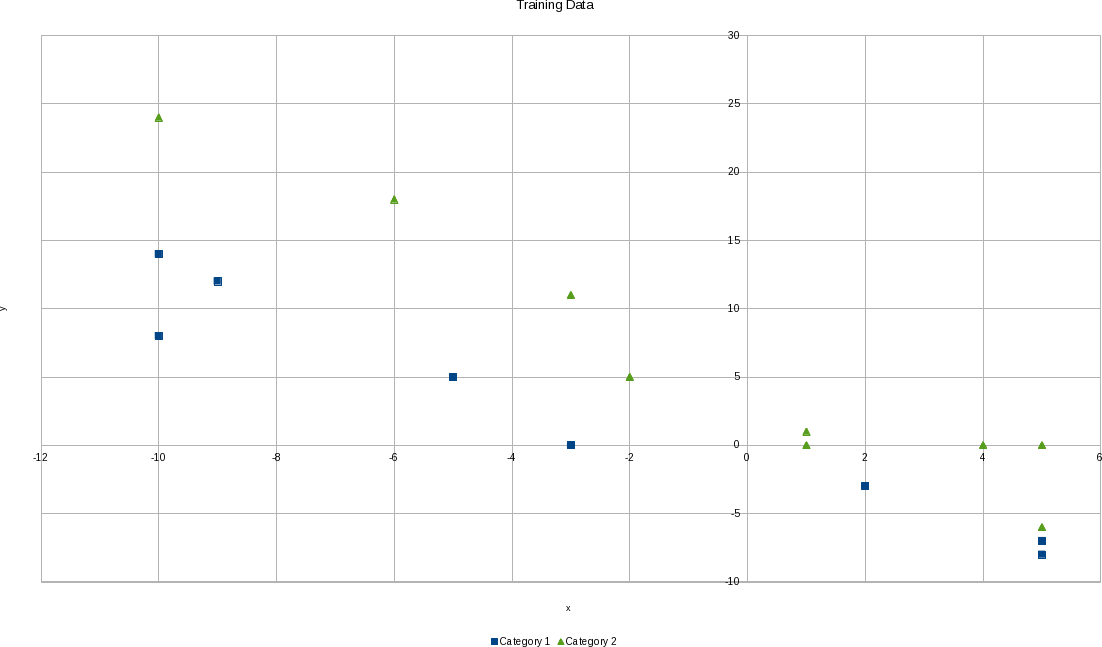
\includegraphics[width=0.7\textwidth]{TrainingValues}
  \caption{Training values for perceptron}
  \label{fig:TrainingValues}
\end{figure}
\begin{figure}[H]
  \centering
  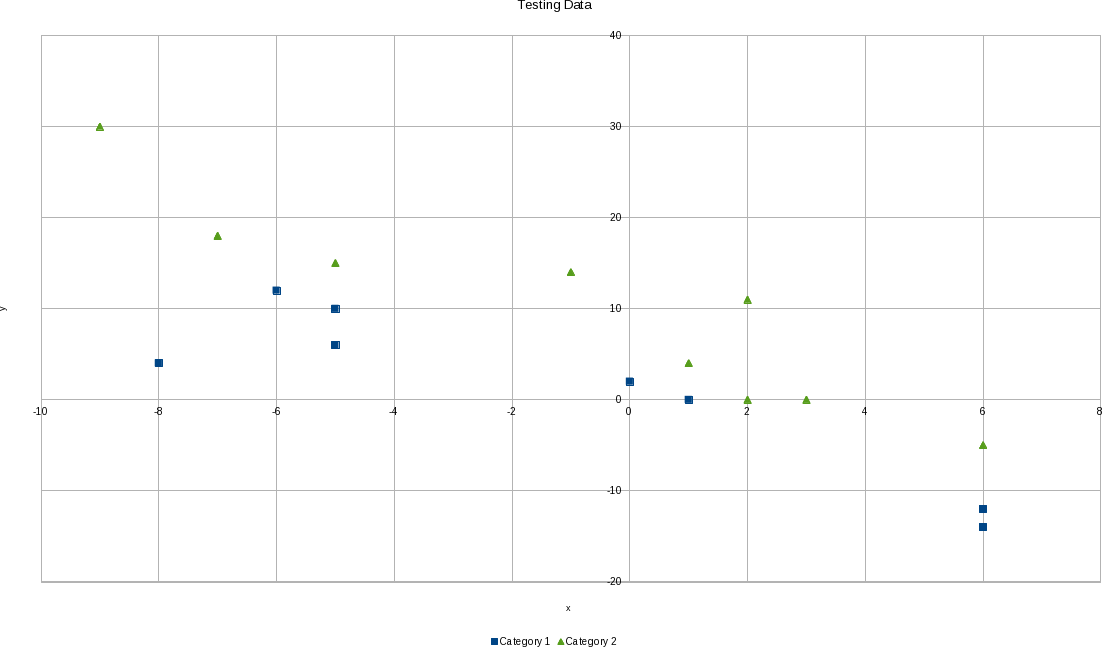
\includegraphics[width=0.7\textwidth]{TestingValues}
  \caption{Testing values for perceptron}
  \label{fig:TestingValues}
\end{figure}

Results:
\begin{verbatim}
Average training error: 0.23529411764705882
Average testing error:  0.29411764705882354
Average training error: 0.11764705882352941
Average testing error:  0.23529411764705882
Average training error: 0.058823529411764705
Average testing error:  0.29411764705882354
Average training error: 0.058823529411764705
Average testing error:  0.23529411764705882
Average training error: 0.0
Average testing error:  0.23529411764705882
Average training error: 0.0
Average testing error:  0.23529411764705882
Average training error: 0.0
Average testing error:  0.23529411764705882
Average training error: 0.0
Average testing error:  0.23529411764705882
Average training error: 0.0
Average testing error:  0.23529411764705882
Average training error: 0.0
Average testing error:  0.23529411764705882
\end{verbatim}
After 10 epochs I can see no more improvements. Graphs showing average error for training and testing sets can be seen in \cref{fig:TrainingErrorGraph,fig:TestingErrorGraph}.
\begin{figure}[H]
  \centering
  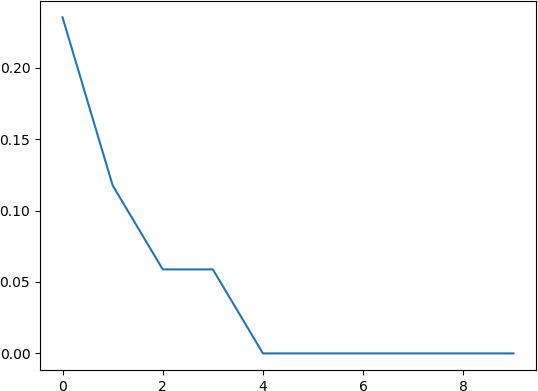
\includegraphics[width=0.7\textwidth]{TrainingErrorGraph}
  \caption{Training errors for perceptron}
  \label{fig:TrainingErrorGraph}
\end{figure}
\begin{figure}[H]
  \centering
  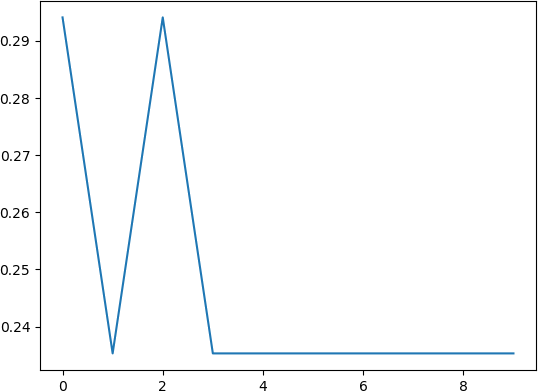
\includegraphics[width=0.7\textwidth]{TestingErrorGraph}
  \caption{Testing errors for perceptron}
  \label{fig:TestingErrorGraph}
\end{figure}

\mysubsection{3}{c}
I need about 4 cycles to minimize the error. Though I need 8 to 10 cycles to minimize the error if I decrease the bias.

\mysubsection{4}{d}
My training error drops to 0, while my testing error drops to 0.235.

\mysubsection{5}{e}
Using Excel I found the regression line between those two sets to have following attributes: y interception = 3.63, x-slope = -1.76. Drawing that as a chart I get following \cref{fig:RegressionLine}.
\begin{figure}[H]
  \centering
  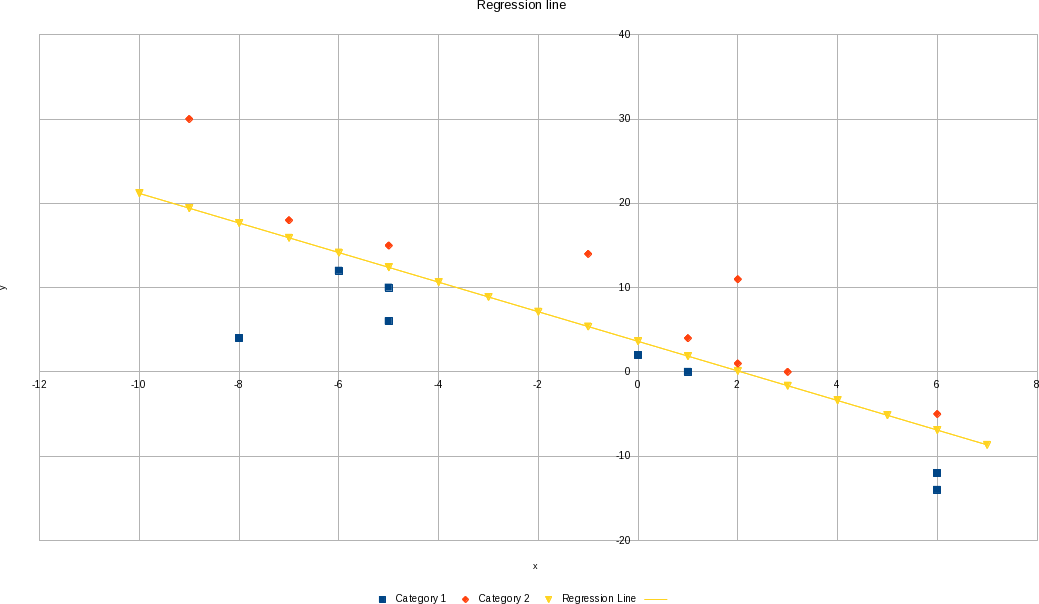
\includegraphics[width=0.7\textwidth]{RegressionLine}
  \caption{Training errors for perceptron using original values}
  \label{fig:RegressionLine}
\end{figure}

\mysubsubsection{6}{f}
Back Propagation Network is able to solve much more complex problems, for example problems where variables are not linearly separable. Given how this is a simple problem with simple numerical values and linearly separated values I have no need for Back Propagation Network.

Though as I have mentioned before I needed to change the values to linearly separate the input values. If I use the values provided in the assignment my perceptor struggles greatly and needs about 40 to 50 epochs to minimize the error. However error does not platau, it instead settles jumping back and forth between two values. As can be seen in \cref{fig:TrainingErrorOriginal,fig:TestingErrorOriginal} below.
\begin{figure}[H]
  \centering
  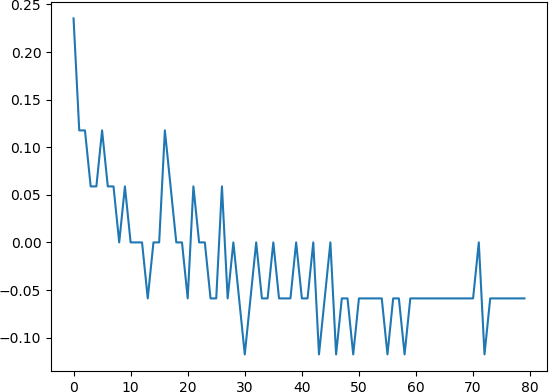
\includegraphics[width=0.7\textwidth]{TrainingErrorOriginal}
  \caption{Training errors for perceptron using original values}
  \label{fig:TrainingErrorOriginal}
\end{figure}
\begin{figure}[H]
  \centering
  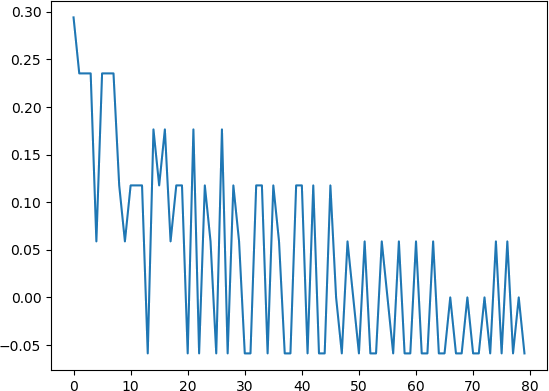
\includegraphics[width=0.7\textwidth]{TestingErrorOriginal}
  \caption{Testing errors for perceptron using original values}
  \label{fig:TestingErrorOriginal}
\end{figure}

\end{document} 